\documentclass{article}
\usepackage{tikz}
\usetikzlibrary{positioning}

\begin{document}

\begin{center}
    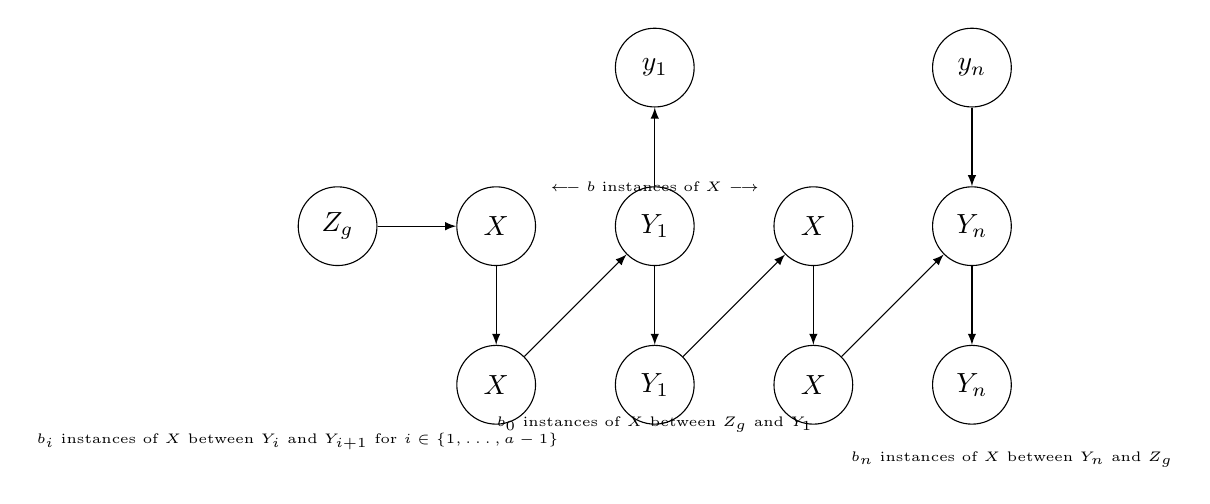
\begin{tikzpicture}[node distance=1cm]
        % Define styles for nodes
        \tikzstyle{vertex}=[circle, draw, minimum size=1cm]
        \tikzstyle{edge}=[draw, -latex]

        % Draw the left and right boxes
        \node[vertex] (Zg_left) {$Z_g$};
        \node[vertex] (X1_left) [right=of Zg_left] {$X$};
        \node[vertex] (X2_left) [below=of X1_left] {$X$};
        \node[vertex] (Y1_left) [right=of X1_left] {$Y_1$};
        \node[vertex] (Y2_left) [below=of Y1_left] {$Y_1$};

        \node[vertex] (X1_right) [right=of Y1_left] {$X$};
        \node[vertex] (X2_right) [below=of X1_right] {$X$};
        \node[vertex] (Y1_right) [right=of X1_right] {$Y_n$};
        \node[vertex] (Y2_right) [below=of Y1_right] {$Y_n$};

        % Draw the connecting edges
        \draw[edge] (Zg_left) -- (X1_left);
        \draw[edge] (X1_left) -- (X2_left);
        \draw[edge] (X2_left) -- (Y1_left);
        \draw[edge] (Y1_left) -- (Y2_left);
        \draw[edge] (Y2_left) -- (X1_right);
        \draw[edge] (X1_right) -- (X2_right);
        \draw[edge] (X2_right) -- (Y1_right);
        \draw[edge] (Y1_right) -- (Y2_right);

        % Add labels
        \node at (current bounding box.north) {\tiny $\longleftarrow b$ instances of $X$ $\longrightarrow$};
        \node at (current bounding box.south) {\tiny $b_0$ instances of $X$ between $Z_g$ and $Y_1$};
        \node at (current bounding box.south west) {\tiny $b_i$ instances of $X$ between $Y_i$ and $Y_{i+1}$ for $i \in \{1,\ldots,a-1\}$};
        \node at (current bounding box.south east) {\tiny $b_n$ instances of $X$ between $Y_n$ and $Z_g$};

        % Draw the middle boxes
        \node[vertex] (Y1_middle) [above=of Y1_left] {$y_1$};
        \node[vertex] (Yn_middle) [above=of Y1_right] {$y_n$};

        % Connect the middle boxes to the left and right boxes
        \draw[edge] (Y1_left) -- (Y1_middle);
        \draw[edge] (Yn_middle) -- (Y1_right);
    \end{tikzpicture}
\end{center}

\caption{Cubic graph \( G^a_g(B) \) where \( B = \{b, b_0, \dots, b_a\} \).}

\end{document}